\documentclass[twoside]{book}

% Packages required by doxygen
\usepackage{fixltx2e}
\usepackage{calc}
\usepackage{doxygen}
\usepackage[export]{adjustbox} % also loads graphicx
\usepackage{graphicx}
\usepackage[utf8]{inputenc}
\usepackage{makeidx}
\usepackage{multicol}
\usepackage{multirow}
\PassOptionsToPackage{warn}{textcomp}
\usepackage{textcomp}
\usepackage[nointegrals]{wasysym}
\usepackage[table]{xcolor}

% Font selection
\usepackage[T1]{fontenc}
\usepackage[scaled=.90]{helvet}
\usepackage{courier}
\usepackage{amssymb}
\usepackage{sectsty}
\renewcommand{\familydefault}{\sfdefault}
\allsectionsfont{%
  \fontseries{bc}\selectfont%
  \color{darkgray}%
}
\renewcommand{\DoxyLabelFont}{%
  \fontseries{bc}\selectfont%
  \color{darkgray}%
}
\newcommand{\+}{\discretionary{\mbox{\scriptsize$\hookleftarrow$}}{}{}}

% Page & text layout
\usepackage{geometry}
\geometry{%
  a4paper,%
  top=2.5cm,%
  bottom=2.5cm,%
  left=2.5cm,%
  right=2.5cm%
}
\tolerance=750
\hfuzz=15pt
\hbadness=750
\setlength{\emergencystretch}{15pt}
\setlength{\parindent}{0cm}
\setlength{\parskip}{3ex plus 2ex minus 2ex}
\makeatletter
\renewcommand{\paragraph}{%
  \@startsection{paragraph}{4}{0ex}{-1.0ex}{1.0ex}{%
    \normalfont\normalsize\bfseries\SS@parafont%
  }%
}
\renewcommand{\subparagraph}{%
  \@startsection{subparagraph}{5}{0ex}{-1.0ex}{1.0ex}{%
    \normalfont\normalsize\bfseries\SS@subparafont%
  }%
}
\makeatother

% Headers & footers
\usepackage{fancyhdr}
\pagestyle{fancyplain}
\fancyhead[LE]{\fancyplain{}{\bfseries\thepage}}
\fancyhead[CE]{\fancyplain{}{}}
\fancyhead[RE]{\fancyplain{}{\bfseries\leftmark}}
\fancyhead[LO]{\fancyplain{}{\bfseries\rightmark}}
\fancyhead[CO]{\fancyplain{}{}}
\fancyhead[RO]{\fancyplain{}{\bfseries\thepage}}
\fancyfoot[LE]{\fancyplain{}{}}
\fancyfoot[CE]{\fancyplain{}{}}
\fancyfoot[RE]{\fancyplain{}{\bfseries\scriptsize Generated by Doxygen }}
\fancyfoot[LO]{\fancyplain{}{\bfseries\scriptsize Generated by Doxygen }}
\fancyfoot[CO]{\fancyplain{}{}}
\fancyfoot[RO]{\fancyplain{}{}}
\renewcommand{\footrulewidth}{0.4pt}
\renewcommand{\chaptermark}[1]{%
  \markboth{#1}{}%
}
\renewcommand{\sectionmark}[1]{%
  \markright{\thesection\ #1}%
}

% Indices & bibliography
\usepackage{natbib}
\usepackage[titles]{tocloft}
\setcounter{tocdepth}{3}
\setcounter{secnumdepth}{5}
\makeindex

% Hyperlinks (required, but should be loaded last)
\usepackage{ifpdf}
\ifpdf
  \usepackage[pdftex,pagebackref=true]{hyperref}
\else
  \usepackage[ps2pdf,pagebackref=true]{hyperref}
\fi
\hypersetup{%
  colorlinks=true,%
  linkcolor=blue,%
  citecolor=blue,%
  unicode%
}

% Custom commands
\newcommand{\clearemptydoublepage}{%
  \newpage{\pagestyle{empty}\cleardoublepage}%
}

\usepackage{caption}
\captionsetup{labelsep=space,justification=centering,font={bf},singlelinecheck=off,skip=4pt,position=top}

%===== C O N T E N T S =====

\begin{document}

% Titlepage & ToC
\hypersetup{pageanchor=false,
             bookmarksnumbered=true,
             pdfencoding=unicode
            }
\pagenumbering{alph}
\begin{titlepage}
\vspace*{7cm}
\begin{center}%
{\Large Minerva }\\
\vspace*{1cm}
{\large Generated by Doxygen 1.8.13}\\
\end{center}
\end{titlepage}
\clearemptydoublepage
\pagenumbering{roman}
\tableofcontents
\clearemptydoublepage
\pagenumbering{arabic}
\hypersetup{pageanchor=true}

%--- Begin generated contents ---
\chapter{minverva}
\label{md__r_e_a_d_m_e}
\Hypertarget{md__r_e_a_d_m_e}
\input{md__r_e_a_d_m_e}
\chapter{Hierarchical Index}
\section{Class Hierarchy}
This inheritance list is sorted roughly, but not completely, alphabetically\+:\begin{DoxyCompactList}
\item \contentsline{section}{minerva\+:\+:foundation\+:\+:allocator}{\pageref{classminerva_1_1foundation_1_1allocator}}{}
\begin{DoxyCompactList}
\item \contentsline{section}{minerva\+:\+:foundation\+:\+:singleton$<$ T $>$}{\pageref{classminerva_1_1foundation_1_1singleton}}{}
\item \contentsline{section}{minerva\+:\+:foundation\+:\+:singleton$<$ texture\+\_\+loader $>$}{\pageref{classminerva_1_1foundation_1_1singleton}}{}
\begin{DoxyCompactList}
\item \contentsline{section}{minerva\+:\+:foundation\+:\+:texture\+\_\+loader}{\pageref{classminerva_1_1foundation_1_1texture__loader}}{}
\end{DoxyCompactList}
\end{DoxyCompactList}
\item \contentsline{section}{minerva\+:\+:foundation\+:\+:core}{\pageref{classminerva_1_1foundation_1_1core}}{}
\item \contentsline{section}{minerva\+:\+:foundation\+:\+:memory\+\_\+tracker\+:\+:memory\+\_\+group}{\pageref{structminerva_1_1foundation_1_1memory__tracker_1_1memory__group}}{}
\item \contentsline{section}{minerva\+:\+:foundation\+:\+:memory\+\_\+tracker\+:\+:memory\+\_\+size\+\_\+count\+\_\+info}{\pageref{structminerva_1_1foundation_1_1memory__tracker_1_1memory__size__count__info}}{}
\item \contentsline{section}{minerva\+:\+:foundation\+:\+:memory\+\_\+tracker}{\pageref{classminerva_1_1foundation_1_1memory__tracker}}{}
\item \contentsline{section}{minerva\+:\+:foundation\+:\+:texture\+\_\+data}{\pageref{structminerva_1_1foundation_1_1texture__data}}{}
\end{DoxyCompactList}

\chapter{Class Index}
\section{Class List}
Here are the classes, structs, unions and interfaces with brief descriptions\+:\begin{DoxyCompactList}
\item\contentsline{section}{\hyperlink{classminerva_1_1foundation_1_1allocator}{minerva\+::foundation\+::allocator} \\*Base class of all objects in minerva }{\pageref{classminerva_1_1foundation_1_1allocator}}{}
\end{DoxyCompactList}

\chapter{File Index}
\section{File List}
Here is a list of all documented files with brief descriptions\+:\begin{DoxyCompactList}
\item\contentsline{section}{/\+Users/apple/\+Work/git/github/minverva/fundation/classes/include/\hyperlink{allocator_8h}{allocator.\+h} \\*Allocator for all objects }{\pageref{allocator_8h}}{}
\item\contentsline{section}{/\+Users/apple/\+Work/git/github/minverva/fundation/classes/include/{\bfseries consts.\+h} }{\pageref{consts_8h}}{}
\item\contentsline{section}{/\+Users/apple/\+Work/git/github/minverva/fundation/classes/include/{\bfseries defines.\+h} }{\pageref{defines_8h}}{}
\end{DoxyCompactList}

\chapter{Class Documentation}
\hypertarget{classminerva_1_1foundation_1_1allocator}{}\section{minerva\+:\+:foundation\+:\+:allocator Class Reference}
\label{classminerva_1_1foundation_1_1allocator}\index{minerva\+::foundation\+::allocator@{minerva\+::foundation\+::allocator}}


base class of all objects in minerva  




{\ttfamily \#include $<$allocator.\+h$>$}

\subsection*{Public Member Functions}
\begin{DoxyCompactItemize}
\item 
\mbox{\Hypertarget{classminerva_1_1foundation_1_1allocator_a1d984a6c7360cac43c6182fc8c27f263}\label{classminerva_1_1foundation_1_1allocator_a1d984a6c7360cac43c6182fc8c27f263}} 
\hyperlink{classminerva_1_1foundation_1_1allocator_a1d984a6c7360cac43c6182fc8c27f263}{allocator} ()
\begin{DoxyCompactList}\small\item\em ctor \end{DoxyCompactList}\item 
\mbox{\Hypertarget{classminerva_1_1foundation_1_1allocator_a1818227b868a680283eb08fbaf2abec9}\label{classminerva_1_1foundation_1_1allocator_a1818227b868a680283eb08fbaf2abec9}} 
\hyperlink{classminerva_1_1foundation_1_1allocator_a1818227b868a680283eb08fbaf2abec9}{$\sim$allocator} ()
\begin{DoxyCompactList}\small\item\em dtor \end{DoxyCompactList}\item 
void $\ast$ \hyperlink{classminerva_1_1foundation_1_1allocator_af693b0cd3bdec3bfdc4885b15f9d04c6}{operator new} (size\+\_\+t size, const char $\ast$file, int line, const char $\ast$function)
\begin{DoxyCompactList}\small\item\em operator new with debug information \end{DoxyCompactList}\item 
void $\ast$ \hyperlink{classminerva_1_1foundation_1_1allocator_a19f76fd74546cc86283694836b55570b}{operator new\mbox{[}$\,$\mbox{]}} (size\+\_\+t size, const char $\ast$file, int line, const char $\ast$function)
\begin{DoxyCompactList}\small\item\em operator new\mbox{[}\mbox{]} with debug information \end{DoxyCompactList}\item 
void \hyperlink{classminerva_1_1foundation_1_1allocator_ae33b6c28ecbd236c7e974ac9270601a8}{operator delete} (void $\ast$ptr)
\begin{DoxyCompactList}\small\item\em operator delete \end{DoxyCompactList}\end{DoxyCompactItemize}


\subsection{Detailed Description}
base class of all objects in minerva 

Base class for override new \& delete function and added tracing method when in debug mode 

\subsection{Member Function Documentation}
\mbox{\Hypertarget{classminerva_1_1foundation_1_1allocator_ae33b6c28ecbd236c7e974ac9270601a8}\label{classminerva_1_1foundation_1_1allocator_ae33b6c28ecbd236c7e974ac9270601a8}} 
\index{minerva\+::foundation\+::allocator@{minerva\+::foundation\+::allocator}!operator delete@{operator delete}}
\index{operator delete@{operator delete}!minerva\+::foundation\+::allocator@{minerva\+::foundation\+::allocator}}
\subsubsection{\texorpdfstring{operator delete()}{operator delete()}}
{\footnotesize\ttfamily void minerva\+::foundation\+::allocator\+::operator delete (\begin{DoxyParamCaption}\item[{void $\ast$}]{ptr }\end{DoxyParamCaption})\hspace{0.3cm}{\ttfamily [inline]}}



operator delete 

free an object, with a switch for tracing purpose


\begin{DoxyParams}[1]{Parameters}
\mbox{\tt in}  & {\em object} & pointer of object \\
\hline
\end{DoxyParams}
\mbox{\Hypertarget{classminerva_1_1foundation_1_1allocator_af693b0cd3bdec3bfdc4885b15f9d04c6}\label{classminerva_1_1foundation_1_1allocator_af693b0cd3bdec3bfdc4885b15f9d04c6}} 
\index{minerva\+::foundation\+::allocator@{minerva\+::foundation\+::allocator}!operator new@{operator new}}
\index{operator new@{operator new}!minerva\+::foundation\+::allocator@{minerva\+::foundation\+::allocator}}
\subsubsection{\texorpdfstring{operator new()}{operator new()}}
{\footnotesize\ttfamily void$\ast$ minerva\+::foundation\+::allocator\+::operator new (\begin{DoxyParamCaption}\item[{size\+\_\+t}]{size,  }\item[{const char $\ast$}]{file,  }\item[{int}]{line,  }\item[{const char $\ast$}]{function }\end{DoxyParamCaption})\hspace{0.3cm}{\ttfamily [inline]}}



operator new with debug information 

only activated on debug mode, with a switch for tracing purpose


\begin{DoxyParams}[1]{Parameters}
\mbox{\tt in}  & {\em size} & object\textquotesingle{}s size \\
\hline
\mbox{\tt in}  & {\em file} & which file the new operator occured \\
\hline
\mbox{\tt in}  & {\em line} & where the new located in the file \\
\hline
\mbox{\tt in}  & {\em function} & the function where the new called \\
\hline
\end{DoxyParams}
\mbox{\Hypertarget{classminerva_1_1foundation_1_1allocator_a19f76fd74546cc86283694836b55570b}\label{classminerva_1_1foundation_1_1allocator_a19f76fd74546cc86283694836b55570b}} 
\index{minerva\+::foundation\+::allocator@{minerva\+::foundation\+::allocator}!operator new\mbox{[}\mbox{]}@{operator new[]}}
\index{operator new\mbox{[}\mbox{]}@{operator new[]}!minerva\+::foundation\+::allocator@{minerva\+::foundation\+::allocator}}
\subsubsection{\texorpdfstring{operator new[]()}{operator new[]()}}
{\footnotesize\ttfamily void$\ast$ minerva\+::foundation\+::allocator\+::operator new\mbox{[}$\,$\mbox{]} (\begin{DoxyParamCaption}\item[{size\+\_\+t}]{size,  }\item[{const char $\ast$}]{file,  }\item[{int}]{line,  }\item[{const char $\ast$}]{function }\end{DoxyParamCaption})\hspace{0.3cm}{\ttfamily [inline]}}



operator new\mbox{[}\mbox{]} with debug information 

only activated on debug mode, with a switch for tracing purpose


\begin{DoxyParams}[1]{Parameters}
\mbox{\tt in}  & {\em size} & object\textquotesingle{}s size \\
\hline
\mbox{\tt in}  & {\em file} & which file the new operator occured \\
\hline
\mbox{\tt in}  & {\em line} & where the new located in the file \\
\hline
\mbox{\tt in}  & {\em function} & the function where the new called \\
\hline
\end{DoxyParams}


The documentation for this class was generated from the following file\+:\begin{DoxyCompactItemize}
\item 
/\+Users/apple/\+Work/git/github/minverva/fundation/classes/include/\hyperlink{allocator_8h}{allocator.\+h}\end{DoxyCompactItemize}

\hypertarget{classminerva_1_1foundation_1_1core}{}\section{minerva\+:\+:foundation\+:\+:core Class Reference}
\label{classminerva_1_1foundation_1_1core}\index{minerva\+::foundation\+::core@{minerva\+::foundation\+::core}}


The documentation for this class was generated from the following file\+:\begin{DoxyCompactItemize}
\item 
foundation/foundation/foundation.\+h\end{DoxyCompactItemize}

\hypertarget{structminerva_1_1foundation_1_1memory__tracker_1_1memory__group}{}\section{minerva\+:\+:foundation\+:\+:memory\+\_\+tracker\+:\+:memory\+\_\+group Struct Reference}
\label{structminerva_1_1foundation_1_1memory__tracker_1_1memory__group}\index{minerva\+::foundation\+::memory\+\_\+tracker\+::memory\+\_\+group@{minerva\+::foundation\+::memory\+\_\+tracker\+::memory\+\_\+group}}


group organized by line, function, size and count  




{\ttfamily \#include $<$memory\+\_\+tracker.\+h$>$}

\subsection*{Public Member Functions}
\begin{DoxyCompactItemize}
\item 
\mbox{\Hypertarget{structminerva_1_1foundation_1_1memory__tracker_1_1memory__group_a0b996e4b95bf6f86bcc6572b73ea5732}\label{structminerva_1_1foundation_1_1memory__tracker_1_1memory__group_a0b996e4b95bf6f86bcc6572b73ea5732}} 
\hyperlink{structminerva_1_1foundation_1_1memory__tracker_1_1memory__group_a0b996e4b95bf6f86bcc6572b73ea5732}{memory\+\_\+group} (std\+::string \&\&funcn)
\begin{DoxyCompactList}\small\item\em ctor for structure \end{DoxyCompactList}\end{DoxyCompactItemize}
\subsection*{Public Attributes}
\begin{DoxyCompactItemize}
\item 
\mbox{\Hypertarget{structminerva_1_1foundation_1_1memory__tracker_1_1memory__group_a13b93feaacbc98de0a5978420897ea29}\label{structminerva_1_1foundation_1_1memory__tracker_1_1memory__group_a13b93feaacbc98de0a5978420897ea29}} 
std\+::string \hyperlink{structminerva_1_1foundation_1_1memory__tracker_1_1memory__group_a13b93feaacbc98de0a5978420897ea29}{function\+\_\+name}
\begin{DoxyCompactList}\small\item\em function \end{DoxyCompactList}\item 
\mbox{\Hypertarget{structminerva_1_1foundation_1_1memory__tracker_1_1memory__group_a3de304ca6ef752b29198b97fde2208f4}\label{structminerva_1_1foundation_1_1memory__tracker_1_1memory__group_a3de304ca6ef752b29198b97fde2208f4}} 
mi\+\_\+vector$<$ \hyperlink{structminerva_1_1foundation_1_1memory__tracker_1_1memory__size__count__info}{memory\+\_\+size\+\_\+count\+\_\+info} $>$ \hyperlink{structminerva_1_1foundation_1_1memory__tracker_1_1memory__group_a3de304ca6ef752b29198b97fde2208f4}{size\+\_\+count\+\_\+array}
\begin{DoxyCompactList}\small\item\em size\&count info for different line\&function \end{DoxyCompactList}\end{DoxyCompactItemize}


\subsection{Detailed Description}
group organized by line, function, size and count 

We organize the memory blocks by a key (function) and it\textquotesingle{}s values. Due to a memory allocation may be occured more than once in a single function, so we use a container to distinguish different allocations, besides, the size may vary even in a same line, for instance, array allocation with different size, so we need to handle this too 

The documentation for this struct was generated from the following file\+:\begin{DoxyCompactItemize}
\item 
foundation/foundation/memory/\hyperlink{memory__tracker_8h}{memory\+\_\+tracker.\+h}\end{DoxyCompactItemize}

\hypertarget{structminerva_1_1foundation_1_1memory__tracker_1_1memory__size__count__info}{}\section{minerva\+:\+:foundation\+:\+:memory\+\_\+tracker\+:\+:memory\+\_\+size\+\_\+count\+\_\+info Struct Reference}
\label{structminerva_1_1foundation_1_1memory__tracker_1_1memory__size__count__info}\index{minerva\+::foundation\+::memory\+\_\+tracker\+::memory\+\_\+size\+\_\+count\+\_\+info@{minerva\+::foundation\+::memory\+\_\+tracker\+::memory\+\_\+size\+\_\+count\+\_\+info}}


size and count structure  




{\ttfamily \#include $<$memory\+\_\+tracker.\+h$>$}

\subsection*{Public Member Functions}
\begin{DoxyCompactItemize}
\item 
\mbox{\Hypertarget{structminerva_1_1foundation_1_1memory__tracker_1_1memory__size__count__info_ab2a5feb1a5c4f7f22c41963e36f6c887}\label{structminerva_1_1foundation_1_1memory__tracker_1_1memory__size__count__info_ab2a5feb1a5c4f7f22c41963e36f6c887}} 
\hyperlink{structminerva_1_1foundation_1_1memory__tracker_1_1memory__size__count__info_ab2a5feb1a5c4f7f22c41963e36f6c887}{memory\+\_\+size\+\_\+count\+\_\+info} (uint line, size\+\_\+t size, uint count)
\begin{DoxyCompactList}\small\item\em ctor for structure \end{DoxyCompactList}\end{DoxyCompactItemize}
\subsection*{Public Attributes}
\begin{DoxyCompactItemize}
\item 
\mbox{\Hypertarget{structminerva_1_1foundation_1_1memory__tracker_1_1memory__size__count__info_a437690ec9d6b6bbd704808bb0005f4c7}\label{structminerva_1_1foundation_1_1memory__tracker_1_1memory__size__count__info_a437690ec9d6b6bbd704808bb0005f4c7}} 
uint \hyperlink{structminerva_1_1foundation_1_1memory__tracker_1_1memory__size__count__info_a437690ec9d6b6bbd704808bb0005f4c7}{n\+\_\+line}
\begin{DoxyCompactList}\small\item\em line of file \end{DoxyCompactList}\item 
\mbox{\Hypertarget{structminerva_1_1foundation_1_1memory__tracker_1_1memory__size__count__info_ab23054ba4ff513298c9beb7b225f503b}\label{structminerva_1_1foundation_1_1memory__tracker_1_1memory__size__count__info_ab23054ba4ff513298c9beb7b225f503b}} 
size\+\_\+t \hyperlink{structminerva_1_1foundation_1_1memory__tracker_1_1memory__size__count__info_ab23054ba4ff513298c9beb7b225f503b}{t\+\_\+size}
\begin{DoxyCompactList}\small\item\em size of each allocation in the same line \end{DoxyCompactList}\item 
\mbox{\Hypertarget{structminerva_1_1foundation_1_1memory__tracker_1_1memory__size__count__info_a85a80b6cc0e3d9573dd8f45fa122ddaa}\label{structminerva_1_1foundation_1_1memory__tracker_1_1memory__size__count__info_a85a80b6cc0e3d9573dd8f45fa122ddaa}} 
uint \hyperlink{structminerva_1_1foundation_1_1memory__tracker_1_1memory__size__count__info_a85a80b6cc0e3d9573dd8f45fa122ddaa}{ui\+\_\+count}
\begin{DoxyCompactList}\small\item\em how many times does it do allocate \end{DoxyCompactList}\end{DoxyCompactItemize}


\subsection{Detailed Description}
size and count structure 

The documentation for this struct was generated from the following file\+:\begin{DoxyCompactItemize}
\item 
foundation/foundation/memory/\hyperlink{memory__tracker_8h}{memory\+\_\+tracker.\+h}\end{DoxyCompactItemize}

\hypertarget{classminerva_1_1foundation_1_1memory__tracker}{}\section{minerva\+:\+:foundation\+:\+:memory\+\_\+tracker Class Reference}
\label{classminerva_1_1foundation_1_1memory__tracker}\index{minerva\+::foundation\+::memory\+\_\+tracker@{minerva\+::foundation\+::memory\+\_\+tracker}}


Tracking memory allocations.  




{\ttfamily \#include $<$memory\+\_\+tracker.\+h$>$}

\subsection*{Classes}
\begin{DoxyCompactItemize}
\item 
struct \hyperlink{structminerva_1_1foundation_1_1memory__tracker_1_1memory__group}{memory\+\_\+group}
\begin{DoxyCompactList}\small\item\em group organized by line, function, size and count \end{DoxyCompactList}\item 
struct \hyperlink{structminerva_1_1foundation_1_1memory__tracker_1_1memory__size__count__info}{memory\+\_\+size\+\_\+count\+\_\+info}
\begin{DoxyCompactList}\small\item\em size and count structure \end{DoxyCompactList}\end{DoxyCompactItemize}
\subsection*{Public Member Functions}
\begin{DoxyCompactItemize}
\item 
\mbox{\Hypertarget{classminerva_1_1foundation_1_1memory__tracker_a40d5d21ff24b82be3a10809780c503ac}\label{classminerva_1_1foundation_1_1memory__tracker_a40d5d21ff24b82be3a10809780c503ac}} 
void \hyperlink{classminerva_1_1foundation_1_1memory__tracker_a40d5d21ff24b82be3a10809780c503ac}{add} (void $\ast$ptr, size\+\_\+t size, const char $\ast$function, uint line)
\begin{DoxyCompactList}\small\item\em add a record \end{DoxyCompactList}\item 
\mbox{\Hypertarget{classminerva_1_1foundation_1_1memory__tracker_ae0e9730e34188b867d82d69bcbaf5277}\label{classminerva_1_1foundation_1_1memory__tracker_ae0e9730e34188b867d82d69bcbaf5277}} 
void \hyperlink{classminerva_1_1foundation_1_1memory__tracker_ae0e9730e34188b867d82d69bcbaf5277}{remove} (void $\ast$ptr)
\begin{DoxyCompactList}\small\item\em remove a record \end{DoxyCompactList}\item 
\mbox{\Hypertarget{classminerva_1_1foundation_1_1memory__tracker_afd1c76896804a25e446d7b80787b727d}\label{classminerva_1_1foundation_1_1memory__tracker_afd1c76896804a25e446d7b80787b727d}} 
void \hyperlink{classminerva_1_1foundation_1_1memory__tracker_afd1c76896804a25e446d7b80787b727d}{output\+\_\+informations} ()
\begin{DoxyCompactList}\small\item\em print allocated memory infomation \end{DoxyCompactList}\end{DoxyCompactItemize}
\subsection*{Static Public Member Functions}
\begin{DoxyCompactItemize}
\item 
\mbox{\Hypertarget{classminerva_1_1foundation_1_1memory__tracker_ab369ca8783692f7f349d4a023cf25fb3}\label{classminerva_1_1foundation_1_1memory__tracker_ab369ca8783692f7f349d4a023cf25fb3}} 
static \hyperlink{classminerva_1_1foundation_1_1memory__tracker}{memory\+\_\+tracker} $\ast$ \hyperlink{classminerva_1_1foundation_1_1memory__tracker_ab369ca8783692f7f349d4a023cf25fb3}{get} ()
\begin{DoxyCompactList}\small\item\em Instance method. \end{DoxyCompactList}\end{DoxyCompactItemize}
\subsection*{Protected Types}
\begin{DoxyCompactItemize}
\item 
\mbox{\Hypertarget{classminerva_1_1foundation_1_1memory__tracker_a5be7a3215edb1bc52e0cbd54b20c51f0}\label{classminerva_1_1foundation_1_1memory__tracker_a5be7a3215edb1bc52e0cbd54b20c51f0}} 
typedef mi\+\_\+vector$<$ \hyperlink{structminerva_1_1foundation_1_1memory__tracker_1_1memory__group}{memory\+\_\+group} $>$ \hyperlink{classminerva_1_1foundation_1_1memory__tracker_a5be7a3215edb1bc52e0cbd54b20c51f0}{memory\+\_\+groups}
\begin{DoxyCompactList}\small\item\em container of memory group \end{DoxyCompactList}\item 
\mbox{\Hypertarget{classminerva_1_1foundation_1_1memory__tracker_a1540e795038843a4a2d7e965b69aee17}\label{classminerva_1_1foundation_1_1memory__tracker_a1540e795038843a4a2d7e965b69aee17}} 
typedef mi\+\_\+unordered\+\_\+multimap$<$ std\+::string, size\+\_\+t $>$ \hyperlink{classminerva_1_1foundation_1_1memory__tracker_a1540e795038843a4a2d7e965b69aee17}{memory\+\_\+search}
\begin{DoxyCompactList}\small\item\em for memory search \end{DoxyCompactList}\item 
typedef mi\+\_\+unordered\+\_\+map$<$ ulong, ullong $>$ \hyperlink{classminerva_1_1foundation_1_1memory__tracker_a1440e17c5c56740dce312e2b49a48199}{pointer\+\_\+search}
\begin{DoxyCompactList}\small\item\em for memory address record \end{DoxyCompactList}\end{DoxyCompactItemize}
\subsection*{Protected Member Functions}
\begin{DoxyCompactItemize}
\item 
\mbox{\Hypertarget{classminerva_1_1foundation_1_1memory__tracker_a821e4d5c9e9e077861d561d918b3218c}\label{classminerva_1_1foundation_1_1memory__tracker_a821e4d5c9e9e077861d561d918b3218c}} 
size\+\_\+t \hyperlink{classminerva_1_1foundation_1_1memory__tracker_a821e4d5c9e9e077861d561d918b3218c}{\+\_\+increase} (size\+\_\+t index, size\+\_\+t size, uint line)
\begin{DoxyCompactList}\small\item\em increase count based on index and size \end{DoxyCompactList}\item 
\mbox{\Hypertarget{classminerva_1_1foundation_1_1memory__tracker_afb9e4a478044a8ceae79b5cccf3dbf0c}\label{classminerva_1_1foundation_1_1memory__tracker_afb9e4a478044a8ceae79b5cccf3dbf0c}} 
void \hyperlink{classminerva_1_1foundation_1_1memory__tracker_afb9e4a478044a8ceae79b5cccf3dbf0c}{\+\_\+decrease} (ullong index)
\begin{DoxyCompactList}\small\item\em decrease count based on index and size \end{DoxyCompactList}\item 
\mbox{\Hypertarget{classminerva_1_1foundation_1_1memory__tracker_af1ca0ea6da700237e944807eee244795}\label{classminerva_1_1foundation_1_1memory__tracker_af1ca0ea6da700237e944807eee244795}} 
size\+\_\+t \hyperlink{classminerva_1_1foundation_1_1memory__tracker_af1ca0ea6da700237e944807eee244795}{\+\_\+get\+\_\+memory\+\_\+group\+\_\+index\+\_\+by\+\_\+name} (const std\+::string \&function\+\_\+name, uint line) const
\begin{DoxyCompactList}\small\item\em finding \hyperlink{structminerva_1_1foundation_1_1memory__tracker_1_1memory__group}{memory\+\_\+group} by filename and line number \end{DoxyCompactList}\end{DoxyCompactItemize}
\subsection*{Protected Attributes}
\begin{DoxyCompactItemize}
\item 
\mbox{\Hypertarget{classminerva_1_1foundation_1_1memory__tracker_a284ff79dd13867f374f438f6a30fc485}\label{classminerva_1_1foundation_1_1memory__tracker_a284ff79dd13867f374f438f6a30fc485}} 
\hyperlink{classminerva_1_1foundation_1_1memory__tracker_a5be7a3215edb1bc52e0cbd54b20c51f0}{memory\+\_\+groups} \hyperlink{classminerva_1_1foundation_1_1memory__tracker_a284ff79dd13867f374f438f6a30fc485}{\+\_\+groups}
\begin{DoxyCompactList}\small\item\em container for memory that allocated \end{DoxyCompactList}\item 
\mbox{\Hypertarget{classminerva_1_1foundation_1_1memory__tracker_adc70e38578d79de1361fc7c3ddda70dd}\label{classminerva_1_1foundation_1_1memory__tracker_adc70e38578d79de1361fc7c3ddda70dd}} 
\hyperlink{classminerva_1_1foundation_1_1memory__tracker_a1540e795038843a4a2d7e965b69aee17}{memory\+\_\+search} \hyperlink{classminerva_1_1foundation_1_1memory__tracker_adc70e38578d79de1361fc7c3ddda70dd}{\+\_\+search}
\begin{DoxyCompactList}\small\item\em used for quickly search \end{DoxyCompactList}\item 
\mbox{\Hypertarget{classminerva_1_1foundation_1_1memory__tracker_a4bd388dba6692aa64e8fbb8f583bcd82}\label{classminerva_1_1foundation_1_1memory__tracker_a4bd388dba6692aa64e8fbb8f583bcd82}} 
\hyperlink{classminerva_1_1foundation_1_1memory__tracker_a1440e17c5c56740dce312e2b49a48199}{pointer\+\_\+search} \hyperlink{classminerva_1_1foundation_1_1memory__tracker_a4bd388dba6692aa64e8fbb8f583bcd82}{\+\_\+pointers}
\begin{DoxyCompactList}\small\item\em pointers \end{DoxyCompactList}\item 
\mbox{\Hypertarget{classminerva_1_1foundation_1_1memory__tracker_a5df2da7a1a0e106c3946982c37b2a499}\label{classminerva_1_1foundation_1_1memory__tracker_a5df2da7a1a0e106c3946982c37b2a499}} 
std\+::mutex \hyperlink{classminerva_1_1foundation_1_1memory__tracker_a5df2da7a1a0e106c3946982c37b2a499}{\+\_\+mutex}
\begin{DoxyCompactList}\small\item\em lock containers \end{DoxyCompactList}\end{DoxyCompactItemize}


\subsection{Detailed Description}
Tracking memory allocations. 

This is a thread-\/safe memory tracker, due to performance concerns, please do not use this class in a release version. 

\subsection{Member Typedef Documentation}
\mbox{\Hypertarget{classminerva_1_1foundation_1_1memory__tracker_a1440e17c5c56740dce312e2b49a48199}\label{classminerva_1_1foundation_1_1memory__tracker_a1440e17c5c56740dce312e2b49a48199}} 
\index{minerva\+::foundation\+::memory\+\_\+tracker@{minerva\+::foundation\+::memory\+\_\+tracker}!pointer\+\_\+search@{pointer\+\_\+search}}
\index{pointer\+\_\+search@{pointer\+\_\+search}!minerva\+::foundation\+::memory\+\_\+tracker@{minerva\+::foundation\+::memory\+\_\+tracker}}
\subsubsection{\texorpdfstring{pointer\+\_\+search}{pointer\_search}}
{\footnotesize\ttfamily typedef mi\+\_\+unordered\+\_\+map$<$ ulong, ullong $>$ \hyperlink{classminerva_1_1foundation_1_1memory__tracker_a1440e17c5c56740dce312e2b49a48199}{minerva\+::foundation\+::memory\+\_\+tracker\+::pointer\+\_\+search}\hspace{0.3cm}{\ttfamily [protected]}}



for memory address record 

for finding purpose, func/index, high-\/32-\/bit are the \+\_\+groups\textquotesingle{} index, low-\/32-\/bit are the size\+\_\+count\+\_\+array\textquotesingle{}s index. 

The documentation for this class was generated from the following files\+:\begin{DoxyCompactItemize}
\item 
foundation/foundation/memory/\hyperlink{memory__tracker_8h}{memory\+\_\+tracker.\+h}\item 
foundation/foundation/memory/memory\+\_\+tracker.\+cpp\end{DoxyCompactItemize}

\hypertarget{classminerva_1_1foundation_1_1singleton}{}\section{minerva\+:\+:foundation\+:\+:singleton$<$ T $>$ Class Template Reference}
\label{classminerva_1_1foundation_1_1singleton}\index{minerva\+::foundation\+::singleton$<$ T $>$@{minerva\+::foundation\+::singleton$<$ T $>$}}


This is a template class.  




{\ttfamily \#include $<$singleton.\+h$>$}

Inheritance diagram for minerva\+:\+:foundation\+:\+:singleton$<$ T $>$\+:\begin{figure}[H]
\begin{center}
\leavevmode
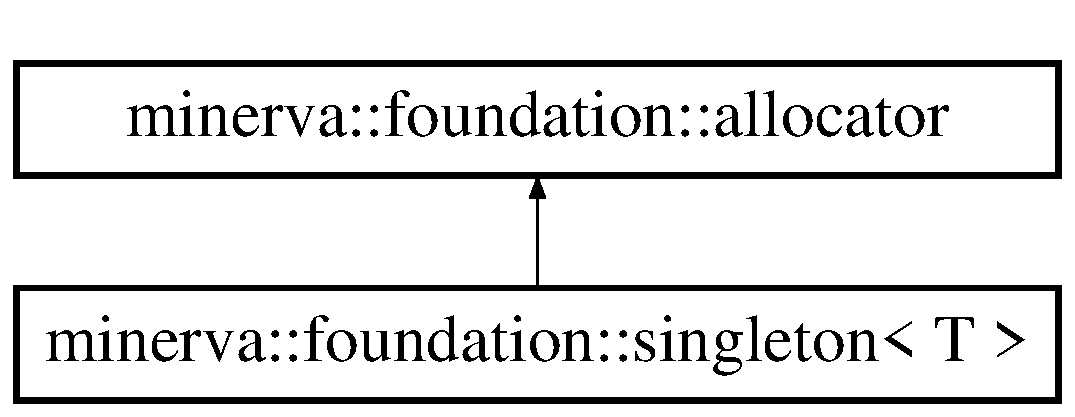
\includegraphics[height=2.000000cm]{classminerva_1_1foundation_1_1singleton}
\end{center}
\end{figure}
\subsection*{Static Public Member Functions}
\begin{DoxyCompactItemize}
\item 
\mbox{\Hypertarget{classminerva_1_1foundation_1_1singleton_afcf49cb2f73ad84c581ae042f14fcfa3}\label{classminerva_1_1foundation_1_1singleton_afcf49cb2f73ad84c581ae042f14fcfa3}} 
static bool \hyperlink{classminerva_1_1foundation_1_1singleton_afcf49cb2f73ad84c581ae042f14fcfa3}{initialize} ()
\begin{DoxyCompactList}\small\item\em Initialize the instance of T. \end{DoxyCompactList}\item 
\mbox{\Hypertarget{classminerva_1_1foundation_1_1singleton_a7dba3de79ff655d663909a7887191cdd}\label{classminerva_1_1foundation_1_1singleton_a7dba3de79ff655d663909a7887191cdd}} 
static void \hyperlink{classminerva_1_1foundation_1_1singleton_a7dba3de79ff655d663909a7887191cdd}{destroy} ()
\begin{DoxyCompactList}\small\item\em Destroy \+\_\+this. \end{DoxyCompactList}\item 
\mbox{\Hypertarget{classminerva_1_1foundation_1_1singleton_a7b0310f5964028ea874b654241bd87fa}\label{classminerva_1_1foundation_1_1singleton_a7b0310f5964028ea874b654241bd87fa}} 
static T $\ast$ \hyperlink{classminerva_1_1foundation_1_1singleton_a7b0310f5964028ea874b654241bd87fa}{get} ()
\begin{DoxyCompactList}\small\item\em Get the instance of T. \end{DoxyCompactList}\end{DoxyCompactItemize}
\subsection*{Protected Member Functions}
\begin{DoxyCompactItemize}
\item 
\mbox{\Hypertarget{classminerva_1_1foundation_1_1singleton_ad300ebe4f0d5ebc93c701667b4275984}\label{classminerva_1_1foundation_1_1singleton_ad300ebe4f0d5ebc93c701667b4275984}} 
\hyperlink{classminerva_1_1foundation_1_1singleton_ad300ebe4f0d5ebc93c701667b4275984}{singleton} ()
\begin{DoxyCompactList}\small\item\em private constructor \end{DoxyCompactList}\end{DoxyCompactItemize}
\subsection*{Additional Inherited Members}


\subsection{Detailed Description}
\subsubsection*{template$<$class T$>$\newline
class minerva\+::foundation\+::singleton$<$ T $>$}

This is a template class. 

T represent the class that need to be singleton 

The documentation for this class was generated from the following file\+:\begin{DoxyCompactItemize}
\item 
foundation/foundation/\hyperlink{singleton_8h}{singleton.\+h}\end{DoxyCompactItemize}

\hypertarget{structminerva_1_1foundation_1_1texture__data}{}\section{minerva\+:\+:foundation\+:\+:texture\+\_\+data Struct Reference}
\label{structminerva_1_1foundation_1_1texture__data}\index{minerva\+::foundation\+::texture\+\_\+data@{minerva\+::foundation\+::texture\+\_\+data}}


texture data loaded from disk  




{\ttfamily \#include $<$texture\+\_\+common.\+h$>$}

\subsection*{Public Attributes}
\begin{DoxyCompactItemize}
\item 
\mbox{\Hypertarget{structminerva_1_1foundation_1_1texture__data_a9d157ba85b70515de6fce6f93e90c6c9}\label{structminerva_1_1foundation_1_1texture__data_a9d157ba85b70515de6fce6f93e90c6c9}} 
uint \hyperlink{structminerva_1_1foundation_1_1texture__data_a9d157ba85b70515de6fce6f93e90c6c9}{format}
\begin{DoxyCompactList}\small\item\em texture format \end{DoxyCompactList}\item 
\mbox{\Hypertarget{structminerva_1_1foundation_1_1texture__data_aa6c5aeb2fdbd76aa859dfffea0ec7274}\label{structminerva_1_1foundation_1_1texture__data_aa6c5aeb2fdbd76aa859dfffea0ec7274}} 
uint \hyperlink{structminerva_1_1foundation_1_1texture__data_aa6c5aeb2fdbd76aa859dfffea0ec7274}{width}
\begin{DoxyCompactList}\small\item\em texture width \end{DoxyCompactList}\item 
\mbox{\Hypertarget{structminerva_1_1foundation_1_1texture__data_a44abed30b09fa739f74d16fe66487867}\label{structminerva_1_1foundation_1_1texture__data_a44abed30b09fa739f74d16fe66487867}} 
uint \hyperlink{structminerva_1_1foundation_1_1texture__data_a44abed30b09fa739f74d16fe66487867}{height}
\begin{DoxyCompactList}\small\item\em texture height \end{DoxyCompactList}\item 
\mbox{\Hypertarget{structminerva_1_1foundation_1_1texture__data_aae8415655c566a326cedfaf2795260a8}\label{structminerva_1_1foundation_1_1texture__data_aae8415655c566a326cedfaf2795260a8}} 
uint \hyperlink{structminerva_1_1foundation_1_1texture__data_aae8415655c566a326cedfaf2795260a8}{mipmap\+\_\+count}
\begin{DoxyCompactList}\small\item\em mipmap count, 0 mean no mimap \end{DoxyCompactList}\item 
\mbox{\Hypertarget{structminerva_1_1foundation_1_1texture__data_a04c929b908e1b4cadb0e8a0d7a212e64}\label{structminerva_1_1foundation_1_1texture__data_a04c929b908e1b4cadb0e8a0d7a212e64}} 
uchar $\ast$ \hyperlink{structminerva_1_1foundation_1_1texture__data_a04c929b908e1b4cadb0e8a0d7a212e64}{buffer}
\begin{DoxyCompactList}\small\item\em texture data \end{DoxyCompactList}\end{DoxyCompactItemize}


\subsection{Detailed Description}
texture data loaded from disk 

The documentation for this struct was generated from the following file\+:\begin{DoxyCompactItemize}
\item 
foundation/foundation/texture/texture\+\_\+common.\+h\end{DoxyCompactItemize}

\hypertarget{classminerva_1_1foundation_1_1texture__loader}{}\section{minerva\+:\+:foundation\+:\+:texture\+\_\+loader Class Reference}
\label{classminerva_1_1foundation_1_1texture__loader}\index{minerva\+::foundation\+::texture\+\_\+loader@{minerva\+::foundation\+::texture\+\_\+loader}}


A global thread-\/safe texture loader.  




{\ttfamily \#include $<$texture\+\_\+loader.\+h$>$}

Inheritance diagram for minerva\+:\+:foundation\+:\+:texture\+\_\+loader\+:\begin{figure}[H]
\begin{center}
\leavevmode
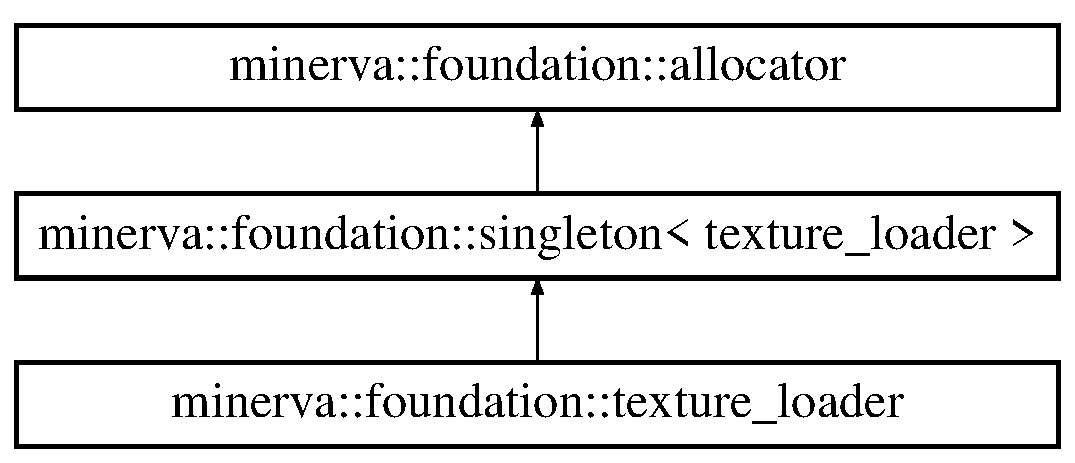
\includegraphics[height=3.000000cm]{classminerva_1_1foundation_1_1texture__loader}
\end{center}
\end{figure}
\subsection*{Public Member Functions}
\begin{DoxyCompactItemize}
\item 
void \hyperlink{classminerva_1_1foundation_1_1texture__loader_a493b46fc8bb2d74195aa5a85db0a725f}{load\+\_\+dds\+\_\+from\+\_\+file\+\_\+no\+\_\+safe} (const std\+::string \&file\+\_\+name, \hyperlink{structminerva_1_1foundation_1_1texture__data}{texture\+\_\+data} $\ast$data)
\begin{DoxyCompactList}\small\item\em Load .dds file, not thread-\/safe. \end{DoxyCompactList}\end{DoxyCompactItemize}
\subsection*{Additional Inherited Members}


\subsection{Detailed Description}
A global thread-\/safe texture loader. 

Thread-\/safe texture loader, support D\+X\+Tn,B\+MP,P\+NG and other popular texture format. 

\subsection{Member Function Documentation}
\mbox{\Hypertarget{classminerva_1_1foundation_1_1texture__loader_a493b46fc8bb2d74195aa5a85db0a725f}\label{classminerva_1_1foundation_1_1texture__loader_a493b46fc8bb2d74195aa5a85db0a725f}} 
\index{minerva\+::foundation\+::texture\+\_\+loader@{minerva\+::foundation\+::texture\+\_\+loader}!load\+\_\+dds\+\_\+from\+\_\+file\+\_\+no\+\_\+safe@{load\+\_\+dds\+\_\+from\+\_\+file\+\_\+no\+\_\+safe}}
\index{load\+\_\+dds\+\_\+from\+\_\+file\+\_\+no\+\_\+safe@{load\+\_\+dds\+\_\+from\+\_\+file\+\_\+no\+\_\+safe}!minerva\+::foundation\+::texture\+\_\+loader@{minerva\+::foundation\+::texture\+\_\+loader}}
\subsubsection{\texorpdfstring{load\+\_\+dds\+\_\+from\+\_\+file\+\_\+no\+\_\+safe()}{load\_dds\_from\_file\_no\_safe()}}
{\footnotesize\ttfamily void minerva\+::foundation\+::texture\+\_\+loader\+::load\+\_\+dds\+\_\+from\+\_\+file\+\_\+no\+\_\+safe (\begin{DoxyParamCaption}\item[{const std\+::string \&}]{file\+\_\+name,  }\item[{\hyperlink{structminerva_1_1foundation_1_1texture__data}{texture\+\_\+data} $\ast$}]{data }\end{DoxyParamCaption})}



Load .dds file, not thread-\/safe. 


\begin{DoxyParams}[1]{Parameters}
\mbox{\tt in}  & {\em file\+\_\+name} & texture\textquotesingle{}s file name. \\
\hline
\mbox{\tt out}  & {\em data} & output data \\
\hline
\end{DoxyParams}


The documentation for this class was generated from the following file\+:\begin{DoxyCompactItemize}
\item 
foundation/foundation/texture/texture\+\_\+loader.\+h\end{DoxyCompactItemize}

\chapter{File Documentation}
\hypertarget{foundation_8cpp}{}\section{foundation/foundation/foundation.cpp File Reference}
\label{foundation_8cpp}\index{foundation/foundation/foundation.\+cpp@{foundation/foundation/foundation.\+cpp}}


initiliaze foundation related classes  


{\ttfamily \#include \char`\"{}foundation.\+h\char`\"{}}\newline


\subsection{Detailed Description}
initiliaze foundation related classes 

\begin{DoxyAuthor}{Author}
jiayi 
\end{DoxyAuthor}
\begin{DoxyDate}{Date}
17/01/2017 
\end{DoxyDate}

\hypertarget{allocator_8h}{}\section{/\+Users/apple/\+Work/git/github/minverva/fundation/classes/include/allocator.h File Reference}
\label{allocator_8h}\index{/\+Users/apple/\+Work/git/github/minverva/fundation/classes/include/allocator.\+h@{/\+Users/apple/\+Work/git/github/minverva/fundation/classes/include/allocator.\+h}}


allocator for all objects  


{\ttfamily \#include $<$memory$>$}\newline
{\ttfamily \#include \char`\"{}consts.\+h\char`\"{}}\newline
\subsection*{Classes}
\begin{DoxyCompactItemize}
\item 
class \hyperlink{classminerva_1_1foundation_1_1allocator}{minerva\+::foundation\+::allocator}
\begin{DoxyCompactList}\small\item\em base class of all objects in minerva \end{DoxyCompactList}\end{DoxyCompactItemize}


\subsection{Detailed Description}
allocator for all objects 

\begin{DoxyAuthor}{Author}
jiayi 
\end{DoxyAuthor}
\begin{DoxyDate}{Date}
14/01/2017 
\end{DoxyDate}

\hypertarget{memory__tracker_8h}{}\section{foundation/foundation/memory/memory\+\_\+tracker.h File Reference}
\label{memory__tracker_8h}\index{foundation/foundation/memory/memory\+\_\+tracker.\+h@{foundation/foundation/memory/memory\+\_\+tracker.\+h}}


tracking memory allocation and deallocation  


{\ttfamily \#include \char`\"{}defines.\+h\char`\"{}}\newline
{\ttfamily \#include \char`\"{}standard\+\_\+libraries/unordered\+\_\+multimap.\+h\char`\"{}}\newline
{\ttfamily \#include \char`\"{}standard\+\_\+libraries/unordered\+\_\+map.\+h\char`\"{}}\newline
{\ttfamily \#include \char`\"{}standard\+\_\+libraries/vector.\+h\char`\"{}}\newline
{\ttfamily \#include $<$mutex$>$}\newline
{\ttfamily \#include $<$string$>$}\newline
\subsection*{Classes}
\begin{DoxyCompactItemize}
\item 
class \hyperlink{classminerva_1_1foundation_1_1memory__tracker}{minerva\+::foundation\+::memory\+\_\+tracker}
\begin{DoxyCompactList}\small\item\em Tracking memory allocations. \end{DoxyCompactList}\item 
struct \hyperlink{structminerva_1_1foundation_1_1memory__tracker_1_1memory__size__count__info}{minerva\+::foundation\+::memory\+\_\+tracker\+::memory\+\_\+size\+\_\+count\+\_\+info}
\begin{DoxyCompactList}\small\item\em size and count structure \end{DoxyCompactList}\item 
struct \hyperlink{structminerva_1_1foundation_1_1memory__tracker_1_1memory__group}{minerva\+::foundation\+::memory\+\_\+tracker\+::memory\+\_\+group}
\begin{DoxyCompactList}\small\item\em group organized by line, function, size and count \end{DoxyCompactList}\end{DoxyCompactItemize}
\subsection*{Macros}
\begin{DoxyCompactItemize}
\item 
\mbox{\Hypertarget{memory__tracker_8h_a568e64c79afcb807a332ce365fd93ebb}\label{memory__tracker_8h_a568e64c79afcb807a332ce365fd93ebb}} 
\#define \hyperlink{memory__tracker_8h_a568e64c79afcb807a332ce365fd93ebb}{the\+\_\+memory\+\_\+tracker}~memory\+\_\+tracker\+::get()
\begin{DoxyCompactList}\small\item\em for short \end{DoxyCompactList}\end{DoxyCompactItemize}


\subsection{Detailed Description}
tracking memory allocation and deallocation 

\begin{DoxyAuthor}{Author}
jiayi 
\end{DoxyAuthor}
\begin{DoxyDate}{Date}
17/01/2017 
\end{DoxyDate}

\hypertarget{singleton_8h}{}\section{foundation/foundation/singleton.h File Reference}
\label{singleton_8h}\index{foundation/foundation/singleton.\+h@{foundation/foundation/singleton.\+h}}


base class for singleton classes  


{\ttfamily \#include \char`\"{}defines.\+h\char`\"{}}\newline
{\ttfamily \#include \char`\"{}memory/allocator.\+h\char`\"{}}\newline
\subsection*{Classes}
\begin{DoxyCompactItemize}
\item 
class \hyperlink{classminerva_1_1foundation_1_1singleton}{minerva\+::foundation\+::singleton$<$ T $>$}
\begin{DoxyCompactList}\small\item\em This is a template class. \end{DoxyCompactList}\end{DoxyCompactItemize}


\subsection{Detailed Description}
base class for singleton classes 

\begin{DoxyAuthor}{Author}
jiayi 
\end{DoxyAuthor}
\begin{DoxyDate}{Date}
17/01/2017 
\end{DoxyDate}

%--- End generated contents ---

% Index
\backmatter
\newpage
\phantomsection
\clearemptydoublepage
\addcontentsline{toc}{chapter}{Index}
\printindex

\end{document}
